\documentclass[11pt,twocolumn]{article}
\usepackage{url}
\usepackage{breakurl}
\usepackage[breaklinks]{hyperref}
\usepackage{graphicx}
\usepackage{float}
\begin{document}

\begin{titlepage} % Suppresses displaying the page number on the title page and the subsequent page counts as page 1
    \newcommand{\HRule}{\rule{\linewidth}{0.5mm}} % Defines a new command for horizontal lines, change thickness here
    
    \center % Centre everything on the page
    
    %------------------------------------------------
    %    Headings
    %------------------------------------------------
    
    \textsc{\LARGE Indiana University - Bloomington}\\[1.5cm] % Main heading such as the name of your university/college
    
    \textsc{\Large Network Science}\\[0.5cm] % Major heading such as course name
        
    %------------------------------------------------
    %    Title
    %------------------------------------------------
    
    \HRule\\[0.4cm]
    
    {\huge\bfseries Measuring Facebook Influence Using Centrality Measures and Community Detection}\\[0.4cm] % Title of your document
    
    \HRule\\[1.5cm]
    
    %------------------------------------------------
    %    Author(s)
    %------------------------------------------------
    
    \begin{minipage}{0.4\textwidth}
        \begin{flushleft}
            \large
            \textit{Authors}\\
            \textsc{Daniel Hinders\newline} % Your name
            \textsc{Nhi Tran} % Your name

        \end{flushleft}


    \end{minipage}
    ~
    \begin{minipage}{0.4\textwidth}
        \begin{flushright}
            \large
            \textit{Professor}\\
            \textsc{Yong-Yeol (YY) Ahn} % Supervisor's name
        \end{flushright}
    \end{minipage}
    
    % If you don't want a supervisor, uncomment the two lines below and comment the code above
    %{\large\textit{Author}}\\
    %John \textsc{Smith} % Your name
    
    %------------------------------------------------
    %    Date
    %------------------------------------------------
    
    \vfill\vfill\vfill % Position the date 3/4 down the remaining page
    
    {\large\today} % Date, change the \today to a set date if you want to be precise
    
    %------------------------------------------------
    %    Logo
    %------------------------------------------------
    
    %\vfill\vfill
    %\includegraphics[width=0.2\textwidth]{placeholder.jpg}\\[1cm] % Include a department/university logo - this will require the graphicx package
     
    %----------------------------------------------------------------------------------------
    
    \vfill % Push the date up 1/4 of the remaining page
    
\end{titlepage}

\title{Measuring Facebook Influence Using Centrality Measures and Community Detection}
\author{Daniel Hinders and Nhi Tran}
\maketitle
\begin{abstract}
Within the past couple decades, social media has become a large part of everybody's life and our society. With the aid of social media, social influence can take place without physical human interaction and allow people to influence each other just by having social media accounts and the ability to access the Internet. After social media became popular, researchers and scientists have been studying the impact of social media using different methods such as surveys, trials, scientific experiments, and so on. Analyzing social media network graphs is another way of studying social media impact that this paper will cover. Given a public dataset of Page to Page network from Facebook in November 2017, multiple network graph measurements and a community detection method will help identify influential Fabebook pages within a network. By understanding the differences between measurements and what information they provide, it will be beneficial to apply similar measurements and analysis methods on other social media network to identify influential nodes.\end{abstract}

\section{Introduction}

With individuals having the ability to influence others anytime from any location anonymously, it is important to be able to identify their power and influential level within a social network to carefully access the impact. Without the ability to identify influential nodes, a network can be too large to study and time-consuming for anyone to get useful information.    


\subsection{Background}

Social media impact has drastically increased its effect on life in the last 10-15 years, the diverse and far reaching impacts cannot be overstated. Russian influence in the 2016 election, the Obama campaign utilizing social media to achieve a decisive victory in 2008 and social media fueling societal change and  upheaval in the middle east and Hong Kong are some of the examples. 

In another realm, corporations spend a massive 11.6 percent \cite{social-media-pricing} average of their marketing through social media indicating vast impact on societies choices and buying habits through social media.  

In the midst of these large organizations and vast movements in social media, there is a fascinating and powerful impact propagated through lone individuals on social media.  A single individual operating as a social media influencer is an existence that has become increasingly common in our societal vernacular. For many, a full time job as a social influencer has become a viable career. 

Understanding all of these social media forces and impacts is important on many levels. Devastating negative ramifications: a nation state subverting democracy by impacting other countries’ elections, hate groups spreading and inciting violence, and webs of misinformation leading to widespread distrust are all reasons alone to understand social media impact and influence. 

\subsection{Motivation and Objectives}

The ultimate purpose of this paper is to analyze a public Facebook Page-to-Page network to identify important nodes and different communities. 

The first objective is to answer the question that will observe the potential differences between multiple centrality measurements that help identify important nodes within a network - Can we simply use degree to identify powerful nodes in a network?


The second objective is to answer the question that will identify the different between a predetermined classification of a network and how likely would the nodes form a community within their own classification - Can we use page type to detect communities?




\subsection{Existing Work}

\paragraph{Existing Work 1 \cite{world-happiness-report-2018}} Text here
   
\paragraph{Existing Work 2 \cite{world-happiness-report-2018}} Text here

\paragraph{Existing Work 3 \cite{world-happiness-report-2018}} Text here


\section{Process and Approaches}

\begin{figure}[hbt!]
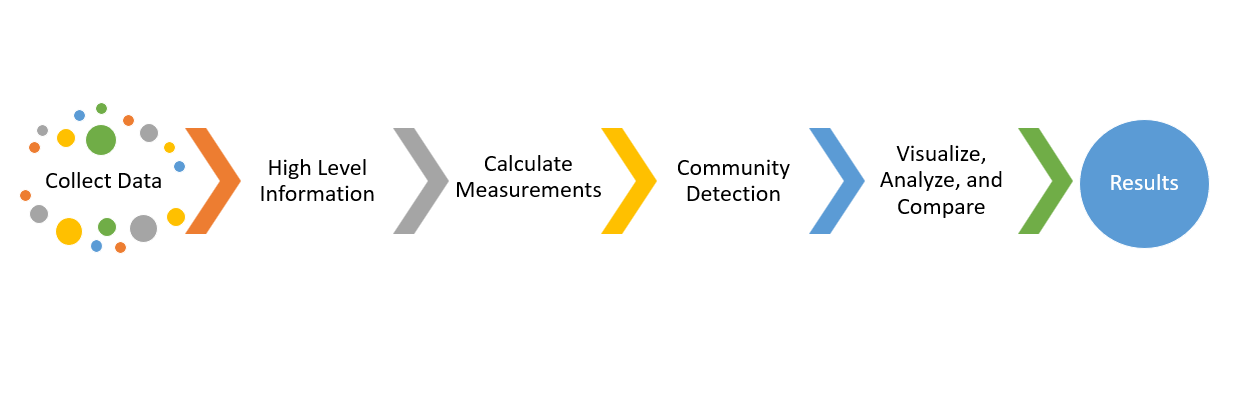
\includegraphics[scale=0.2]{process_flow.PNG} 
\caption{High Level Process}
\end{figure}

\textbf{Figure 1} identifies the steps that are necessary to complete the objectives of this report. Data are collected from Stanford Network Analysis Project. Once the data are collected, the next would be to clean up the network graph, perform high level analysis, calculations, detection community method. Then, all findings will be analyzed, visualized, and compared to get final results.

\subsection{Collecting Data}

\paragraph{Dataset \cite{page-page-network-ds}}
The dataset is November 2017 Facebook Large Page-Page Network from Stanford Network Analysis Project \cite{page-page-network-ds}. The dataset is a compressed zip file that contains the following files :
\begin{itemize}
\item\textbf{\texttt{musae\_facebook\_edges.csv}} – File that contains all edges between pages
\item\textbf{\texttt{musae\_facebook\_features.json}} – JSON file that contains features of the nodes - this file will not be used.
\item\textbf{\texttt{musae\_facebook\_target.csv}} - File that contains list of node ids, page names, and page types.
\end{itemize}

Each edge represents a mutual like between pages and each node is a Facebook page. There are four categories classifies for the Facebook pages: governmental organizations, politicians, television shows and companies. The raw data contains 22,470 nodes and 171,002 edges. 

\subsection{Data Cleaning and High Level Information}

\paragraph{Tools}
The following software and tools were used to perform the analysis:
\begin{itemize}
\item \textbf{Python and Python Packages} - Python packages include Networkx, Pandas, and Matplotlib
\item \textbf{Jupyter Notebook}
\item \textbf{Gephi} - visualization and analysis tool for network graph
\end{itemize}

\paragraph{Cleanup}


\paragraph{High Level Information} 


\subsection{Calculate Measurements }

\subsubsection{Betweenness Centrality} 

\subsubsection{Closeness Centrality}

\subsubsection{Eigenvector Centrality} 
 
\subsection{Community Detection -Modularity}

\subsection{Visualize, Analyze and Compare}


\section{Discussion}


\section{Conclusion}


\section{Acknowledgment}
\section{References}
\bibliography{references} 
\bibliographystyle{ieeetr}
\end{document}
